In this section, we will look at the high-level design of our implementation. We will define the individual components in our
implementation and show how they are connected and how data flows between them.

\subsection{Design}
Our implementation has three important parts, data pre-processor, scene graph generator and query handler. The query handler will also visualise
the answers to the query. In the \cref{fig:system_desgin} you can see the pictorial representation of the three parts as boxes and the connections depict the data flow.
\begin{figure}[ht!]
    \centering
    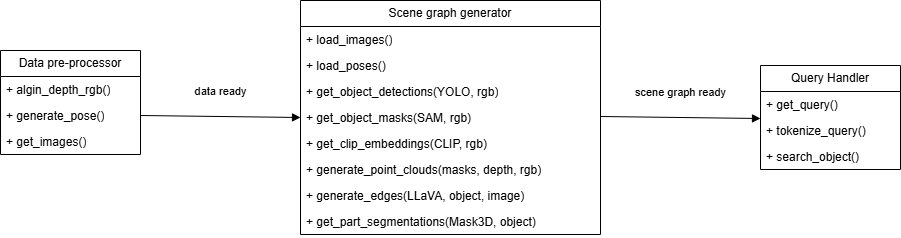
\includegraphics[width=\textwidth]{content/images/Design.png}
    \caption{System design}
    \label{fig:system_desgin}
\end{figure}

We will dive deep into the details of each component one by one. First, we will look at the data pre-processor, next the scene graph generator and finally 
the query handler.

\subsubsection{Data pre-processor}
The data pre-processor is responsible for transforming the raw data from various sources into the format expected by ConceptGraphs. 
ConceptGraphs expects a sequence of RGB-D images and camera poses. Therefore, we need a data pre-processor that can handle various formats of data
and parse them into the expected one.  We mainly focus on data from robots and the cameras mounted on the robots, due to the fact that our system's end goal 
is to assist the robot in task fulfilment. 
Therefore, we will focus on rosbag and .mkv files for RGB-D image sequences. The reason for considering these two data formats is that during our experiments
we will have access to only rosbags and .mkv files obtained from Intel Realsense camera and Femto Bolt by ORBBEC respectively. Moreover, .rosbag is a widely used format in robotics.
The data pre-processor will parse the rosbags and .mkv files  and get a sequence of aligned RGB-D images. 
The RGB and D images must be aligned. The reason for requiring alignment is, that the scene graph 
generator will detect objects from RGB images and from the corresponding depth images it will generate the point clouds and assign colours from 
the RGB images. Thus, alignment is necessary for avoiding wrong colours and malformed objects. \cref{chap:k7} provides the detailed 
implementation point cloud generation. 
Further, the data pre-processor will also be responsible for loading the camera poses. The camera poses can either be absent or be in 
a different format. In the first case, we will use SfM software for obtaining poses from RGB images. In the second case, we will need to
ensure that all the poses are transformed into camera-to-world coordinates which is expected by concept graphs.
\begin{figure}[ht!]
    \centering
    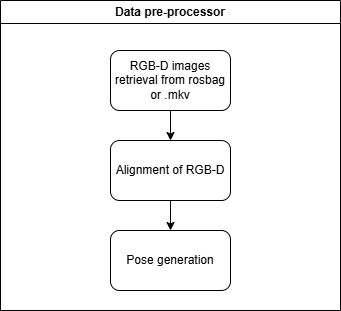
\includegraphics[width=0.5\textwidth]{content/images/DataPreProcessorDesign.png}
    \caption{Internal components of data pre-processor}
    \label{fig:dataPreprocessor}
\end{figure}
In the \cref{fig:dataPreprocessor}, we can see the sub-components of the data preprocessor.

\subsubsection{Scene graph generator}
The scene graph generation is the central component in our system that handles computationally heavy workloads. Therefore, it makes sense to have an 
in-depth look at this particular component. The scene graph generator is responsible for taking RGB-D image sequences and poses as an input and giving queryable scene graphs
as an output. The final scene graph must be able to handle text queries and return a functional interactive element or an object as an answer to the query. \\
\begin{figure}[ht!]
    \centering
    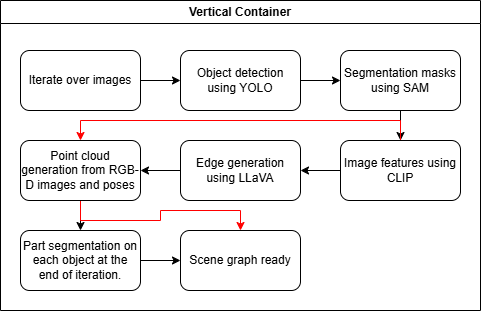
\includegraphics[width=0.5\textwidth]{content/images/SceneGraphGenerator.png}
    \caption{Internal components of scene graph generator}
    \label{fig:sceneGrahpGenerator}
\end{figure}
To generate a scene graph from a set of images we will take the aid of four machine learning models, LLaVA, SAM, YOLO and CLIP. First, we will use YOLO to detect 
objects from given RGB images, YOLO provides bounding boxes and class labels for each detected object. Later, we will employ SAM to get the mask for these detected 
objects, by passing the image and the bounding box to SAM, it will segment out the exact mask for the desired object. We will pass the same image to CLIP
in order to get textual embedding for the image, these embeddings will be used later while querying to find similarities between objects and the query. 
Each object generated from this pipeline will be passed to a VLM like LLaVA to get spatial relationships (edges) between the objects detected. Finally,
we will generate the point cloud for each object using the masks from SAM, the depth values from D images and camera poses for each image. This point cloud
will be passed to a neural network or a transformer to perform part segmentation and segment out functional interactive elements. This way a scene graph will be generated where objects will be
the nodes for this graph and the spatial relationships will be the edges. The scene graph will be then passed to the next component for handling queries.
The tasks of edge generation and part segmentation can be skipped to enable faster scene graph generation, 
this is depicted by red lines in the \cref{fig:sceneGrahpGenerator}.
\subsubsection{Query handler}
This is the last component in our system as depicted in \cref{fig:queryHandler}. It will take a textual query as an input and return a functional element or an object as an answer to the query. The central
part of this component is the CLIP model which will tokenize the input query and then find the most similar objects from the scene graph. The similarities are found 
by finding the cosine similarities between the input query and all the text embeddings generated for each object in the scene graph in the last component using CLIP.
The object with the most similarity is returned as the most probable output, with the remaining objects given weights according to the probabilities. A heat map is 
generated using these probabilities and displayed as a scene graph.\\
\begin{figure}[ht!]
    \centering
    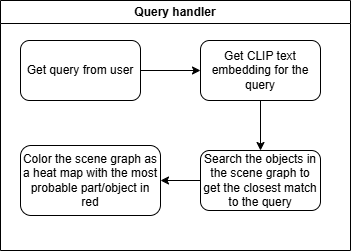
\includegraphics[width=0.5\textwidth]{content/images/QueryHandler.png}
    \caption{Internal components of query handler}
    \label{fig:queryHandler}
\end{figure}

In conclusion, this was the overall design of our proposed system. These are three main components namely, data pre-processor, scene graph generator and query handler. 
The data flow between the components is given in the figure and is linear. Next, we will look at the plan to implement this design, test it and get results.
